\begin{figure}[ht]
\begin{subfigure}{.5\textwidth}
  \centering
  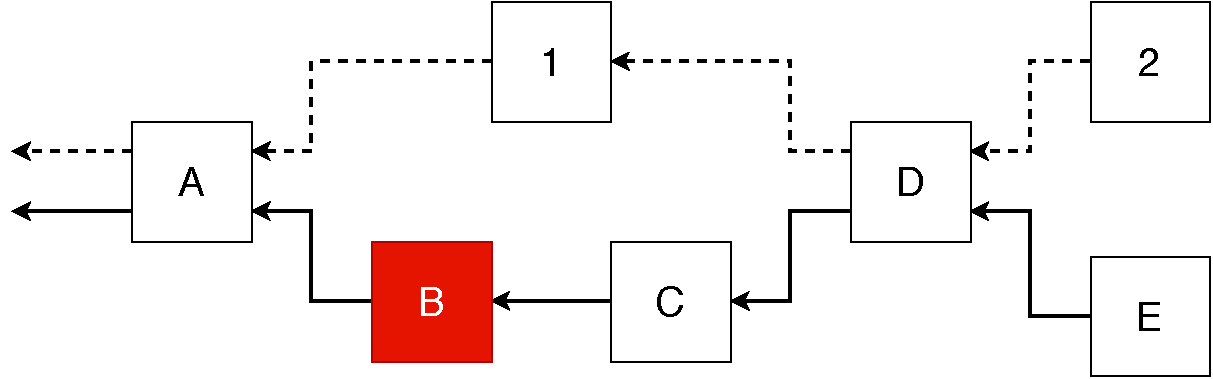
\includegraphics[width=6cm]{../images/Subset_1.pdf}
  \caption{Valid $\pi_{cont}$ DAG+ancestors}
  \label{figure:before__subset}
\end{subfigure}
\begin{subfigure}{.5\textwidth}
  \centering
  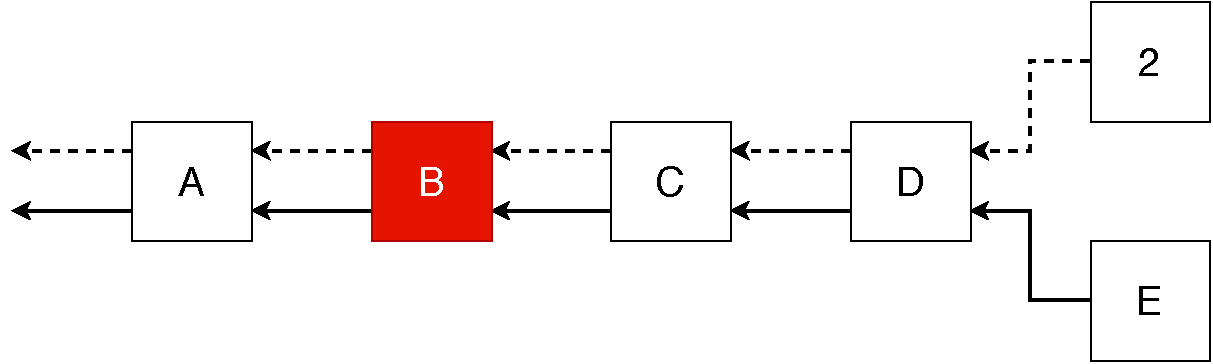
\includegraphics[width=6cm]{../images/Subset_2.pdf}
  \caption{Valid $\pi_{cont}$ using subset}
  \label{figure:after_subset}
\end{subfigure}

\caption{ The red block is the block of interest. The blocks connected with
    solid lines indicate $\pi_{exist}$ and blocks connected with dashed lines
    indicate $\pi_{cont}$. In (a), an adversary can dispatch a flawed proof
    that skips the block of interest.  $\pi_{exits}$ and $\pi_{cont}$ are
aggregated in the  DAG, which is traversed to discover best proof. In (b), the
proofs are linearly iterated to determine if $\pi_{exist}\{:\textrm{LCA}\}
\subseteq \pi_{cont}\{:\textrm{LCA} \}$ }
\label{fig:fig}
\end{figure}
